\documentclass[conference,compsoc]{IEEEtran}



% *** CITATION PACKAGES ***
%
\ifCLASSOPTIONcompsoc
  % IEEE Computer Society needs nocompress option
  % requires cite.sty v4.0 or later (November 2003)
  \usepackage[nocompress]{cite}
\else
  % normal IEEE
  \usepackage{cite}
\fi
% cite.sty was written by Donald Arseneau
% V1.6 and later of IEEEtran pre-defines the format of the cite.sty package

%######### citações modelo abnt 2 ############
\usepackage[num]{abntex2cite}


% *** GRAPHICS RELATED PACKAGES ***
%
\ifCLASSINFOpdf
   \usepackage[pdftex]{graphicx}
  % declare the path(s) where your graphic files are
   \graphicspath{{../pdf/}{../jpeg/}}
  % and their extensions so you won't have to specify these with
  % every instance of \includegraphics
   \DeclareGraphicsExtensions{.pdf,.jpeg,.png}
\else
  % or other class option (dvipsone, dvipdf, if not using dvips). graphicx
  % will default to the driver specified in the system graphics.cfg if no
  % driver is specified.
   \usepackage[dvips]{graphicx}
  % declare the path(s) where your graphic files are
   \graphicspath{{../eps/}}
  % and their extensions so you won't have to specify these with
  % every instance of \includegraphics
   \DeclareGraphicsExtensions{.eps}
\fi

\usepackage{graphicx} % para EPS
\usepackage{subfig}

% correct bad hyphenation here
\hyphenation{op-tical net-works semi-conduc-tor}

% Acentuação Português do Brasil
\usepackage[utf8]{inputenc}

% Permite que o \LaTeX\ fale em português
\usepackage[brazil]{babel}

%hiperlink de Internet
\usepackage[pdftex]{hyperref}


% Conta o número de páginas
\usepackage{lastpage}
\usepackage{setspace}
\pagestyle{plain}

% escrevendo algoritmos
\usepackage[portuguese,ruled,linesnumbered]{algorithm2e}

\begin{document}
%

\title{Minerando dados em grandes quantidades - \textit{Big Data}: SURVEY}


% author names and affiliations
% use a multiple column layout for up to three different
% affiliations
\author{\IEEEauthorblockN{Othon L. T. Oliveira}
\IEEEauthorblockA{Mestrando em Engenharia de Sistemas\\
Universidade de Pernambuco\\
Email: olto@ecomp.poli.br}
\and
\IEEEauthorblockN{Fernando B. L. Neto}
\IEEEauthorblockA{Universidade de Pernambuco\\PhD - UK\\
Email: fbln@ecomp.poli.br}
}

% conference papers do not typically use \thanks and this command
% is locked out in conference mode. If really needed, such as for
% the acknowledgment of grants, issue a \IEEEoverridecommandlockouts
% after \documentclass


% make the title area
\maketitle

% As a general rule, do not put math, special symbols or citations
% in the abstract
\begin{abstract}
Este artigo pretende fazer uma explanação de um novo paradigma, o da informação ilimitada, conhecido como ``Big Data'' e propor uma solução para recuperação de informação para grandes espaços de buscas. Atrelado a este paradigma e reforçando o conceito de que uma nova onda está à frente da Internet, onde coisas se conectam entre si, conhecida como Internet das Coisas ou \textit{Internet of Thigs} (IoT). A Internet das coisas é também conhecido como a ``terceira onda da Internet''; onde computadores conectados a eletrodomésticos; telefones celulares ligados à semáforos, recebem informações sobre o tempo, acidentes e congestionamento e passam essas informação ao carro, que avisa o condutor o que está à frente. Conectar esses novos ``atores'' ou coisas que interagem com os atores humanos é necessário minerar as informações da Internet das coisas, transformando-os em dados para extrair-lhes informação relevante a fim de se aplicar na solução dos problemas do dia a dia.
\end{abstract}

\vspace{0.1cm}

\textit{\textbf{Palavras-chave: Big Data, Mapear e Reduzir, Hadoop, Enxame de robôs, Inteligência em enxames, Aprendizado em profundidade, Aprendizado de máquina, Otimização por enxame de partículas, Otimização por enxame de formigas, Pesquisa por cardume de peixes, Logística, Roteamento }
}.

\vspace{0.1cm}

\textit{Abstract -- This paper intends to make an explanation of a new paradigm, the paradigm of unlimited information known as "Big Data" and to propose a solution for information retrieval for large spaces searches. Coupled to this paradigm and, reinforcing the concept that a new wave lies ahead for the Internet, where things connect with things, we are not as well known Internet of Things   or simply IoT. The IoT is also known as the "third wave of the Internet," the acronym is confirmed because something like computers connected to home appliances, mobile phones connected to the traffic lights, getting weather information, accidents and congestion and to pass this information to the car, which warns the driver what's ahead. This is the reality that approaching and we intend to analyze in this article how the new players, things, interact with traditional actors humans to solve problems of day by day.
}

\textit{Keywords: Big Data, Map Reduce, Hadoop, Swarm Robotics, Swarm Intelligence, Deep Learning, Machine Learning, Particle Swarm Optimization, Ant Colony Optimization, Fish School Search, Logistic, Routing
}.



% For peer review papers, you can put extra information on the cover
% page as needed:
% \ifCLASSOPTIONpeerreview
% \begin{center} \bfseries EDICS Category: 3-BBND \end{center}
% \fi
%
% For peerreview papers, this IEEEtran command inserts a page break and
% creates the second title. It will be ignored for other modes.
\IEEEpeerreviewmaketitle



\section{Introdução}

Inferir sobre algum assunto agora poderá ser coisa do passado. Astrônomos atualizam suas descobertas numa base de 
dados disponíveis para outros utilizarem, as ciências biológicas agora tem tradição em depositar seus avanços 
científicos em repositórios públicos, redes sociais estão focadas na Web; Facebook, 
LinkedIn, Microsoft, Tweeter e Yahoo sobrevivem coletando informações e repassando-as as empresas de telemarketing, 
empresas de comércio eletrônico como Amazon, Submarino, Americanas.com, Magazine Luíza, utilizam essas informações 
para vender mais e melhor, artigos científicos dos mais variados assuntos, das mais variadas áreas alimentam, 
todos os dias,  com milhões de informações os \textit{Data Centers}, isso é o \textit{Big Data}.


Para fazer frente a esse novo paradigma e extrair informações com eficiência novas abordagem algorítmica se faz necessário. 
As técnicas tradicionais de busca não são eficientes para resolver muitos problemas com grande complexidade, i.e. ordens de grandeza 
dantes inimagináveis, especialmente as que possuem complexidade exponenciais, geradas por explosões combinatórias, felizmente, 
muitos desses problemas não-triviais são eficientemente resolvidos por soluções naturais \cite{Swarm_Medeiros}.

Para resolver a problemática da explosão combinatória das informações são desenvolvidas técnicas para reduzir o tempo de busca, 
tornando os custos computacionais mais aceitáveis, na medida que não exploram todas as possibilidades no caminho até a 
solução procurada, somente o caminho curto onde é mais provável de se encontrar a solução, a essa técnica dá-se o nome de heurística.



\section{Objetivos}

Este artigo ``Survey'' tem como objetivo a priori mapear as mais diversas tecnologias empregadas para analisar à problemática do ``Big Data'' e seus paradigmas apresentados atualmente, extrair informações e conhecimentos, analisando as técnicas de Inteligência Artificial mais empregadas nesse campo do conhecimento científico.
Como objetivo a posteriori propor uma solução à logística de cargas aplicada à realidade brasileira, objetivando assim uma alternativa ao traçado de rotas determinísticas, inspirado em buscas no ``Big Data''.

Para executarmos este \textit{Survey}, foram feitas coletas de dados entre os meses de 

\section{Plano de execução do Survey}

Primeiramente definidas as seguintes etapas:

\begin{enumerate}
 \item[A.] Coleta dos dados;
 \item[B.] Seleção dos artigos; 
 \item[C.] Escolha dos Filtros;
 \item[D.] Leitura dos artigos.
\end{enumerate}

\subsection{Detalhamento das etapas}

\begin{enumerate}
 \item[A.] Coleta dos dados\\
 Para coletar os dados foram escolhidas sete (7) palavras chaves com relevância ao tema dentro do meio ambiente da pesquisa, destacamos:
  \begin{itemize}
    \item “Data Mining and Swarm Intelligence”
    \item “Data Mining Big Data”
    \item “Data Mining Swarm Robotics”
    \item “Deep Learning”
	\item “Hadoop Map Reduce in Big Data”    
    \item "Machine Learning"
    \item “Map Reduce Big Data”
  \end{itemize}


 De posse das palavras-chave foram criadas planilhas, onde cada folha dessa planilha é representada por uma palavra chave. 
 Incluiu-se no mínimo 30 artigos para cada planilha. 
 Pretendeu-se, com essa arquitetura, construir rapidamente gráficos das mais diferentes matizes, tais como:
  \begin{itemize}
    \item Base pesquisada;
    \item Data da publicação do artigo;
    \item Aceito ou rejeitado;
    \item Título do artigo;
    \item País de origem do artigo.
  \end{itemize}

  Uma das ferramentas utilizadas para extrair os dados referentes às palavras-chave foi o programa Mendeley, especializado
  em extrair dados de arquivos pdfs como os artigos, dissertações e teses. O Mendeley oferece uma opção para gerar dados 
  extraídos em formato estruturado do tipo XML. A priori foi utilizado para gerar as planilhas, contudo, foi excluída essa
  opção por não trazer grandes ganhos, talvez se fossem criadas macros para tratar esses arquivos XML ficassem mais ``limpos''
  pois o que mais foi relevante para esta fase do Survey formaram as colunas de cada planilha:
  A figura 1 mostra como está a planilha-Survey até este momento;
  
 
  \begin{figure}[!ht]
  \centering %\centering % para centralizarmos a figura
  \caption{Planilha}
  \flushright
  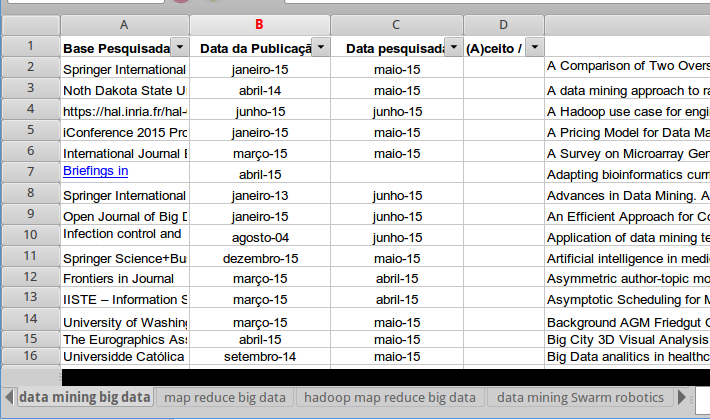
\includegraphics[width=0.4\textwidth]{Figuras/PlanilhaSrvey.png}
%  \label{Fig 1}
  \end{figure}
  
  \item[B.] Seleção dos artigos\\
  A seleção dos artigos foi primeiramente escolhida de forma qualitativa, pelas mais recentes publicações, 
  dos últimos 5 anos, para ser mais exato entre 2010 e 2015. O segundo critério de seleção foi pelo órgão publicizador, 
  haja vista os mais conhecidos tais como IEEE, Elsevier, Springer, e deles todos os jornais pertinentes, contudo
  outras fontes foram consideradas como universidades, seminários mais conhecidos na área.

  Outro critério de seleção foi o quantitativo. Para isso foi estabelecido o mínimo de 30 (trinta artigos) por palavra chave.
  Dessa forma procuramos aproximar os dados coletados da distribuição normal padrão que por razões evidentes está amplamente
  tabelada e é suprida por quase todos os software para construtores de gráficos.\\

  \item[C.] Critérios de Inclusão/Exclusão \\
  O critério de inclusão e exclusão foi baseado na leitura dos ``abstracts'' dos artigos. 
  Devido a algumas palavras estarem muito na ``moda'' são citados em muitos artigos, apesar de conterem as palavras chaves,
  mesmo assim não traziam qualquer relevância para a pesquisa. Dessa forma foi criada uma pasta chamada ``Rejeitados'' 
  para onde foram movidos esses artigos.\\
  Outro critério de exclusão foi a data mais antiga, anteriormente à 2010, com alguma exceção dos artigos clássicos da área.\\

  \item[D.] Leitura dos artigos \\
  A leitura dos artigo iniciou-se tão logo terminaram os critérios de de Inclusão/Exclusão.
  Foram selecionados cerca de 100 artigos para serem lidos, não excetuando-se excluir mais algum que por ventura não 
  tenham ficados ``presos'' na etapa anterior (C), dos filtros.
  Segue uma tabela com as datas do plano de execução
  
  \begin{table}[htbp]
  \scriptsize
  \centering
  \caption{Datas do Survey}
  \begin{tabular}{|p{18mm}|p{8mm}|p{8mm}|p{8mm}|}
  \hline
  Data & A-Coleta & B-Seleção & C-Filtros \\
  \hline
  Abril a Junho & X & -- & -- \\ \hline
  Junho e Julho & -- & X & X \\ \hline
  Agosto & -- & -- & X \\ \hline

  \end{tabular}
  \end{table}


\end{enumerate}

\section{A Internet}

Uma \textit{Internetwork} ou simplesmente internet é a conexão entre mais de uma rede e hoje em dia a maioria das redes se encontram conectadas.  A Internet é um sistema de \textit{internetwork} organizado e estruturado, a mais notável das internets, uma colaboração de mais de centenas de milhares de redes. Já ``World Wide Web'' (WWW) é apenas um dos muitos serviços que funcionam dentro da Internet. 

O acesso à Internet está condicionado a Provedores de Acesso (ISP), que se classificam em internacionais, que conectam países; nacionais (\textit{backbones} criadas e mantidas por empresas especializados) ; regionais ligadas a outros ISPs, normalmente têm taxas de transmissão menores; e locais que se conectam a ISP regionais ou nacionais e oferecem serviços de conexão a usuários finais.


\begin{figure}[!h]
\centering
%\centering % para centralizarmos a figura
\caption{Internet}
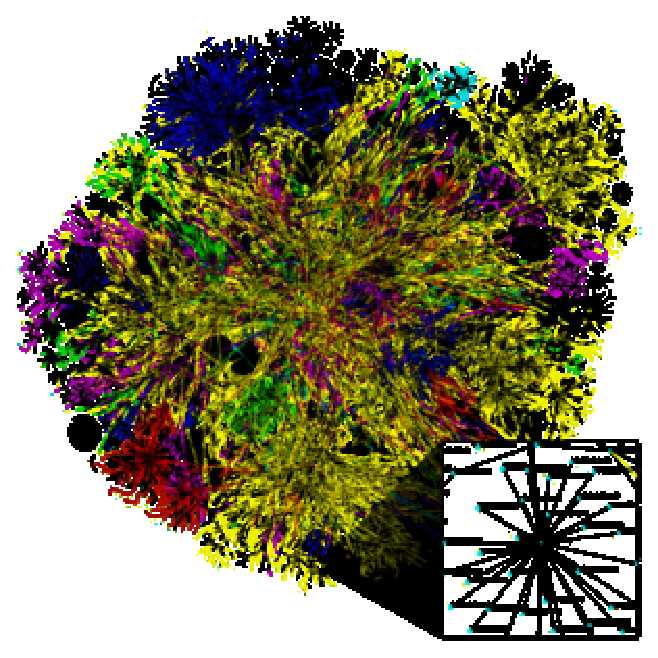
\includegraphics[width=50mm]{Figuras/internet_map.eps}
%\label{figura 2}
\end{figure}



\subsection{Redes de dispositivos conectados}
% no \IEEEPARstart
Uma rede é um conjunto de dispositivos (nós) conectados por links (caminho de transferência) de comunicação.  Um nó pode ser um computador, uma impressora ou outro dispositivo de envio e/ou recepção de dados, que estejam conectados a outro nó da rede \cite{Forouzan}.

Por mais simples e menor que seja, três critérios são considerados os mais importantes que uma rede deve atender: Desempenho, que envolve a capacidade de vazão (througput) e o atraso (delay); Confiabilidade, que envolve o tempo de recuperação quando falha e sua robustez caso haja alguma catástrofe; e Segurança, que envolve proteção ao acesso de dados e proteção contra danos e perdas \cite{Forouzan} \cite{Specialski}.



\section{Big data}

"Em 2010 empresas e usuários armazenaram mais de 13 exabytes de novos dados" \cite{bigdataQualquerUm}.

O paradigma dos 5 V’s exemplifica o Big data, este pode ser descrito como: 

\begin{enumerate}
	\item[1 --]Volume de dados;
	\item[2 --]Velocidade para acessar esses dados;
	\item[3 --]Variedade de informações;
	\item[4 --]Veracidade nos dados encontrados;
	\item[5 --]Valor atribuído aos dados.
\end{enumerate}
  
Dentre as mais diversas ferramentas encontradas destacamos Map Reduce, da ``framework'' Hadoop, por ser de livre uso ``freeware'' e ter grande tolerância `a falhas e fácil implementação, talvez explique a opção de baixo custo para a maioria das empresas e pesquisadores.
A tecnologia congênere, desenvolvida pelo Google ``Google File System'' também tem seu destaque. Essas são as mais conhecidas dos ``aventureiros'' que estão desbravando o Big Data. Não será tarefa trivial inferir e desenvolver novas ferramentas para o Big Data pois este tem 
assumido, nos mais recentes anos proporções gigantescas como descrito na tabela 1

%Tabela 1

\begin{table}[!ht]
\scriptsize
\centering
\caption{Volume de dados no mundo}
\begin{tabular}{|p{6mm}|p{5mm}|p{16mm}|p{8mm}|}
\hline
Ano & Qtd & Unidade & Múltiplo \\
\hline
2000 & 800 & terabytes – TB & $10^{12}$ \\ \hline

2006 & 160 & petabytes – PB & $10^{15}$ \\ \hline

2009 & 500 & exabytes – EB & $10^{18}$ \\ \hline

2012 & 2,7 & zettabytes – ZB & $10^{21}$ \\ \hline

2020 & 35 & yottabytes – YB & $10^{24}$ \\ \hline

\end{tabular}
\end{table}

Atrelada a essa produção massiva de dados, uma nova onda está sendo vislumbrada, é chamada de ``A terceira onda da Internet''
, onde coisas se conectam com coisas; produtos nas gôndolas do supermercado com um novo tipo de etiqueta se conectam a uma 
leitora de radio frequência à alguns metros de distância, contabilizando o total do estoque em segundos; o consumidor leva 
seus produtos escolhidos ao caixa desse supermercado, pagando a conta sem precisar retirar qualquer produto do carrinho. 
Ao introduzir esses produtos na geladeira, será possível saber quando expira a data de validade de determinados produtos, sem 
precisar abri-la, e quando acabarem esses produtos, a própria geladeira informará ao supermercado a falta deles, reservando 
o próximo rol de compras. Assim será essa onda de coisas conectadas, chamada de Internet das Coisas ou \textit{Internet of Things} (IoT),
que fará com que os dados no \textit{Big Data} sofram explosão combinatória de informações multiplicando exponencialmente as dimensões deste.


As redes sociais são um arcabouço de informações sobre todo tipo de assunto vivenciado pelas pessoas, inclusive situações que dizem respeito ao nosso ambiente de pesquisa.
O cenário abaixo, encontrado numa rede social, exemplifica a sequência de informações retiradas do Twitter.
O Twitter é uma rede social, onde os usuários escrevem num pequeno espaço com cerca de 140 caracteres, os mais diversos assuntos. A ideia inicial do Twitter era que se comportasse como um ``SMS da Internet'' \cite{Twitter2015}. As informações são enviadas aos usuários, conhecidas como twittes, em tempo real e, também enviadas aos usuários seguidores que tenham assinado para recebê-las. A seguir pode-se verificar uma sequência de twittes da Polícia Rodoviária Federal de Santa Catarina:

\begin{figure}[!ht]
\caption{Twitter	}
	\subfloat[Twitte - 1 \label{subfig-1:dummy}]{%
		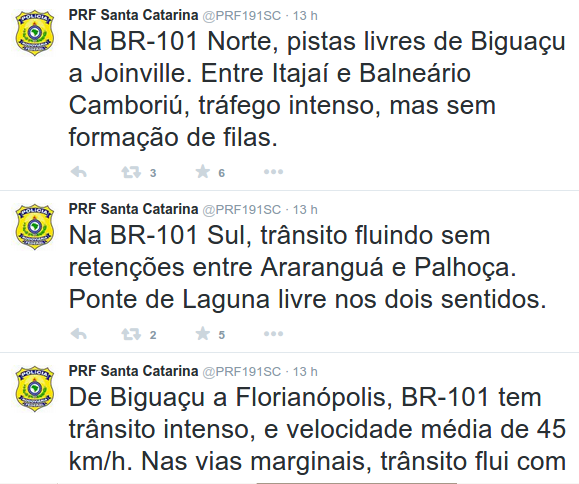
\includegraphics[width=80mm, height=70mm]{Figuras/twittePRF.png}
	}
	\quad \quad \quad \quad
	\subfloat[Twitte - 2\label{subfig-2:dummy}]{%
		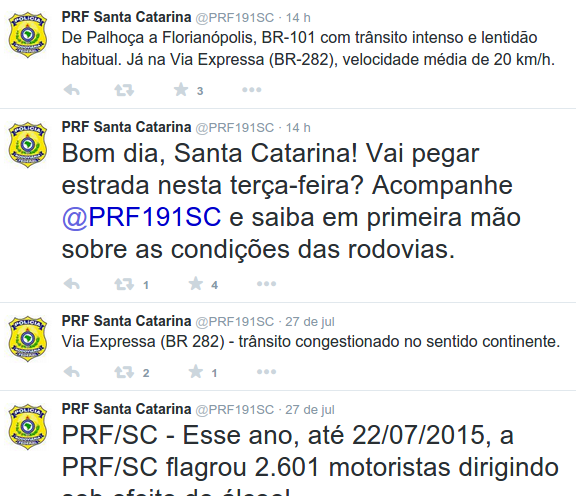
\includegraphics[width=80mm, height=70mm]{Figuras/twittePRF2.png}
	}
	\label{fig:twitter}
\end{figure}

A Polícia Rodoviária Federal de Santa Catarina, disponibilizou às 13hs através do canal @PRF191SC, informações relevantes sobre o trânsito naquela localidade, 
num universo temporal variado, por exemplo: entre Itajaí e Balneário Camboriú o transito está intenso, isso sugere que a frota de caminhões que acompanhamos até este local deva ter uma
rota alternativa, caso persista esta situação por muito tempo. No primeiro twitte da segunda coluna em Via Expressa (BR 282) trânsito lento com 
velocidade de 20km/h praticamente congestionado, novamente sugere que devamos ``pensar'' numa rota alternativa, caso esse congestionamento persista por muito tempo.

Outra rede social conhecida pelos condutores de veículos é o Waze. O Waze é um aplicativo de navegação para o trânsito, funciona em aparelhos celulares e tablets. Os utilizadores desse aplicativo são conhecidos como wazers, os wazers compartilham informações sobre o trânsito, em tempo real. Contudo as informações somente estão disponíveis no momento em que são postadas pelos utilizadores por um período de tempo pequeno, caso não hajam utilizadores trafegando pelas vias ou esses utilizadores não tenham disponibilidade em postar informações, não há o que se compartilhadar.
Outra problema levantado com o waze é que; caso não haja conexão à Internet não há como acessar os dados dos wazers, para navegação.

Além dos dados que chegam ao \textit{Big Data} através das redes sociais, o trânsito das grandes cidades têm disponíveis câmeras de monitoramento do trânsito nos semáforos, alguns com cobertura
por canais de televisão, câmaras de segurança próximos às rodovias também coletam informações, tudo em tempo real. Os dados desses dispositívos geralente são gravados sendo conhecidos como \textit{stream} de dados. 
Esses \textit{streams} podem estar disponibilizados na Internet em sítios eletrônicos especialmente construídos para isso, como o ``vejaaovivo''
\footnote{\textit{http://vejoaovivo.com.br} sítio eletrônico onde encontram-se imagens de câmeras de trânsito em tempo real} e outros.

Os dados disponibilizados pelos diversos meios de comunicação não estão em formato que possam ser utilizados imediatamente, precisam antes serem processados. Esses dados não processados são conhecidos como ``dados frios''.
O processo de tratar as informações, retirando-lhes o ``lixo''; transformando dados ``frios'' em dados ``quentes'', é um processo que tem um custo temporal elevado, devido ao volume dos dados.

Para trabalhar com os dados do Big Data foi criado um tipo arquitetura para computadores trabalharem em conjunto formando um \textit{cluster} essa arquitetura é conhecida como \textit{filesystem}\footnote{\textit{Filesystem}. ou sistema de arquivos, referem-se à forma como os dados são armazenados, organizados e acessados, pelo sistema operacional, em cada partição no disco (ou no disco inteiro)}.

O goolgle é o maior ator do \textit{Big Data}, ele desenvolveu um modelo computacional para pesquisas na Web, e tem apresentado o uso eficiente da técnica MapReduce com modelos de programação combinados com tabelas conhecidas como BigTable. Introduziu o Google File System \cite{Filesystem}. 

Outros grupos de pesquisadores desenvolveram Hadoop Distributed File System (HDFS) que é hoje o sistema de arquivos para Big Data mais utilizado.\cite{Lange2015}


\section{Hadoop -- MapReduce}

Hadoop MapReduce é uma técnica recente, especialmente, projetado para o processamento de grandes conjuntos de dados distribuídos. Hadoop nasceu do Apache. O Apache é um servidor Web, o tal como o Hadoop. Servidores Web são computadores especialmente dedicados a traduzir programas feitos para Internet em página da Internet as quais pessoas possam ler, quando conectam-se `a Internet. MapReduce é um modelo de programação para expressar cálculo distribuído em quantidade maciça de
dados e uma estrutura de execução para dados em larga escala e processamento em clusters de servidores. Foi originalmente desenvolvido pela Google e construído sobre o bem-conhecido
princípios em paralelo e processamento distribuído.
O Hadoop é a implementação de código aberto do MapReduce escrito em java que fornece, tolerância a falhas, escalável e confiável técnica de computação distribuída.
O configurar o ambiente Hadoop envolve um grande número de parâmetros que são essenciais para alcançar um excelente desempenho. Ele permite que desenvolveres de aplicações distribuídas sem qualquer conhecimento possam programar computadores. 
Um "Valor" e uma "chave" formam um par de dados, isso é a estrutura básica de dados do MapReduce. 
Chaves e valores podem ser da forma de dados primitivos; como inteiros, ponto flutuante,  e bytes brutos ou podem ser estruturas arbitrárias e complexas (listas, tuplas matriz associativa, e outras)


\subsection{Hadoop - Map Reduce - Big Data}\label{arte:palavraChave:HadoopMapReduce}

O \textit{Big Data}, devido à sua natureza, foi definido como o paradigma dos 5 V's entre as grandezas: \textbf{Volume}, \textbf{Velocidade}, \textbf{Variedade}, \textbf{Veracidade} e \textbf{Valor}.
O roteiro seguido pela informação desde o local onde é produzida até onde 
possa ser utilizada é exemplificado na imagem a seguir:

\begin{figure}[ht]
\centering
\caption{Big Data e Arquitetura Haddop}
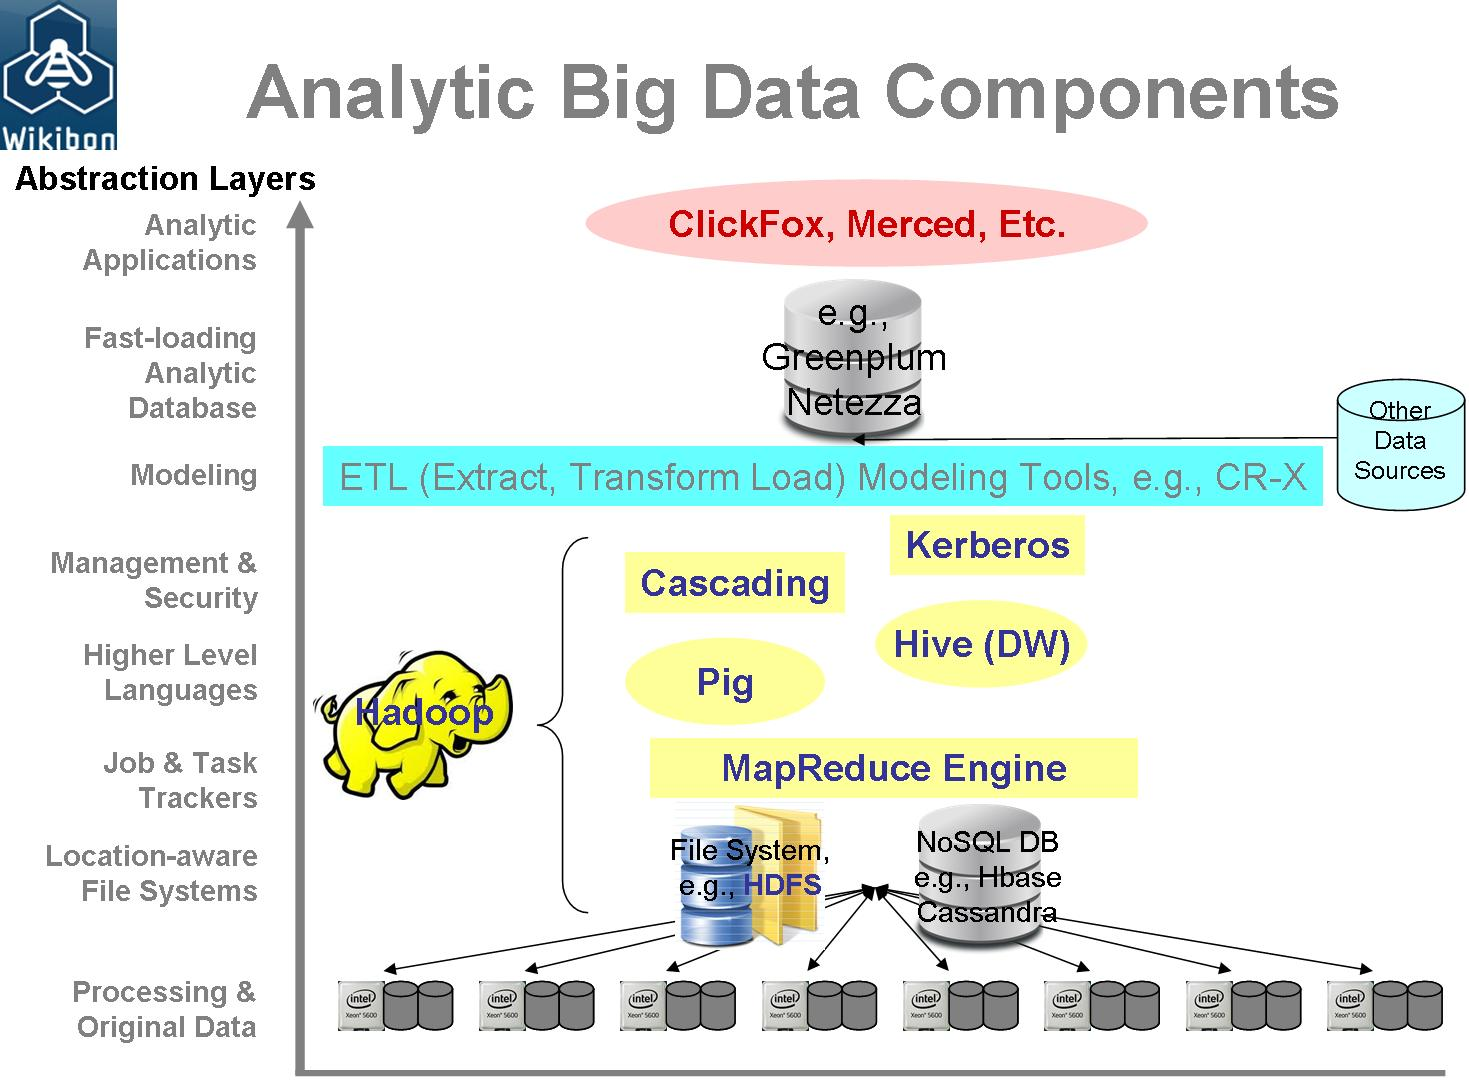
\includegraphics[width=80mm, height=80mm]{Figuras/BigDataComponents.jpg}
\end{figure}

A camada mais baixa da imagem, onde se lê \textit{Processing \& Original Data} é a origem do \textit{Big Data}, onde estão os dados ``frios''. Entre as camadas \textit{Location-aware File Systems} e \textit{Management \& Security} é o roteiro seguido pela informação para ser trasformada em dados ``quentes''. A tecnologia utilizada, para tratar os dados poderá ser o Apache Hadoop ou similar, devido ao baixo custo de implementação e por ser uma tecnologia aberta, de livre utilização, conhecida como \textit{Open Source}. O Haddop é uma arquitetura de milhares de computadores interligados e espalhados e pela Internet. Esses computadores são especializados em extrair dados do \textit{Big Data} e transformá-los em dados relevantes (quentes). \cite{Conejero2015}

O Haddop funciona com um agrupamento em paralelo desses computadores, conhecido como \textit{cluster}. Esse \textit{cluster} tem a característica de grande escalabilidade; em torno de 3 000 computadores na operação de Map, dependendo da construção, e tolerância a falhas; quando um computador do \textit{cluster} fica inoperante  ``cai'', os dados são salvos em outro computador. A estrutura de diretórios do Hadoop é conhecida como \textit{Hadoop File System} (HDFS). O HDFS foi especialmente construído para lidar com as características descritas anteriormente.



\subsection{Map Reduce - Big Data}\label{arte:palavraChave:MapReduceBigData}

O Map-Reduce é uma técnica conhecida desde a linguagem Lisp, que permite Mapear (Map) um conjunto de informações como palavras, imagens, paginas na Internet através do agrupamentos de milhares de computadores conhecido como \textit{cluster} e mesclar essas informação conhecida como reduzir (Reduce) conforme um par de informações \{ chave:valor \} .  
O Hadoop implementa o paradigma MapReduce

A imagem a seguir exemplifica a técnica Map-Reduce:

\begin{figure}[ht]
\centering
\caption{Técnica Map-Reduce}
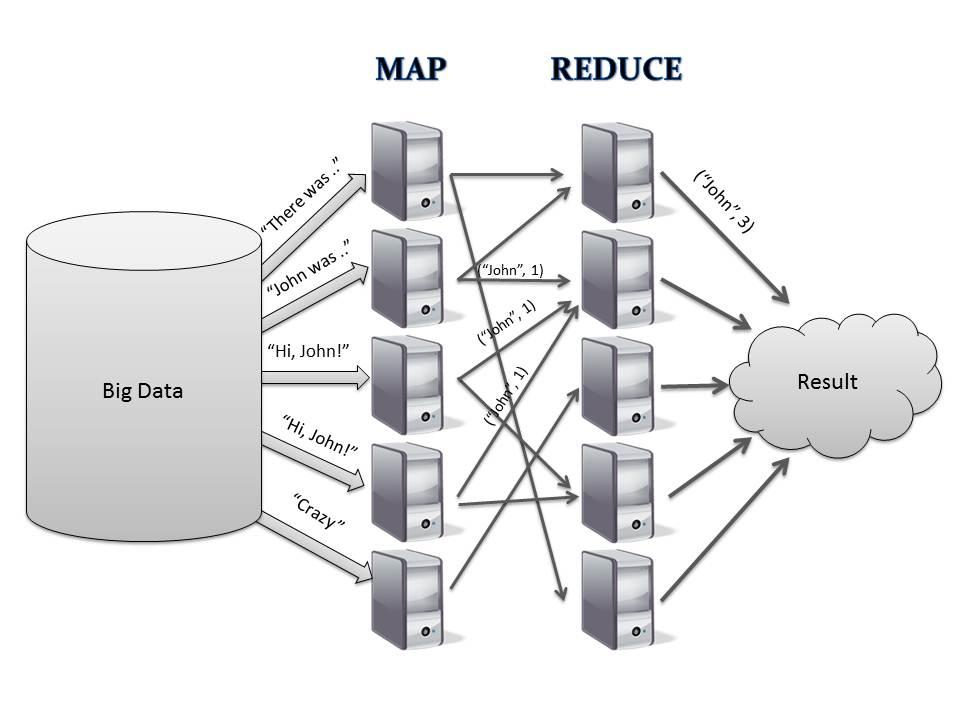
\includegraphics[width=100mm, height=80mm]{Figuras/MapReduce.jpg}
\end{figure}

Durante a operação de ``Map'' podem estar envolvidos \textit{clusters} de até 3.000 computadores ``espalhados'' pela Internet, caso seja utilizada a infraestrutura Hadoop sem virtualização. Na etapa de ``Recude'' o \textit{cluster} cai consideravelmente, contudo o consumo de energia nessas duas etapas consideravelmente alto. \cite{Conejero2015}
Este modelo de Map-Reduce, é um modelo de computação paralelizada proposto pelo Google para ser utilizado na Internet \cite{Dean2008}.

Muitas técnicas tem sido utilizadas para executar a operação de MAP, até virtualização de máquinas, contudo o grande poder do MapReduce está no \textit{cluster} que é implementado com arquitetura em nuvem \textit{Cloud Computing} onde os computadores com \textit{File System} HDFS se comunicam entre si para formar um agrupamento.


\{aqui tirar do artigo: A Modified Key Partitioning for BigData Using MapReduce in Hadoop\}

\section{Data Mining}

Técnicas de mineração de dados trabalham com dados estruturados, para poder extrair informações relevantes.
Um dos maiores problemas na extração de informações são os ``missing data'' ou dados ausentes. Para contornar os dados ausentes exitem varias técnicas como preenchimento dos dados através de técnicas de inteligencia artificial.

O caminho da extração dos dados até sua mineração e por fim extração de conhecimento é longa, na figura a seguir temos um exemplo desse caminho:

\begin{figure}[!ht]
\centering
\caption{Minerando dados no Big Data}
\flushleft
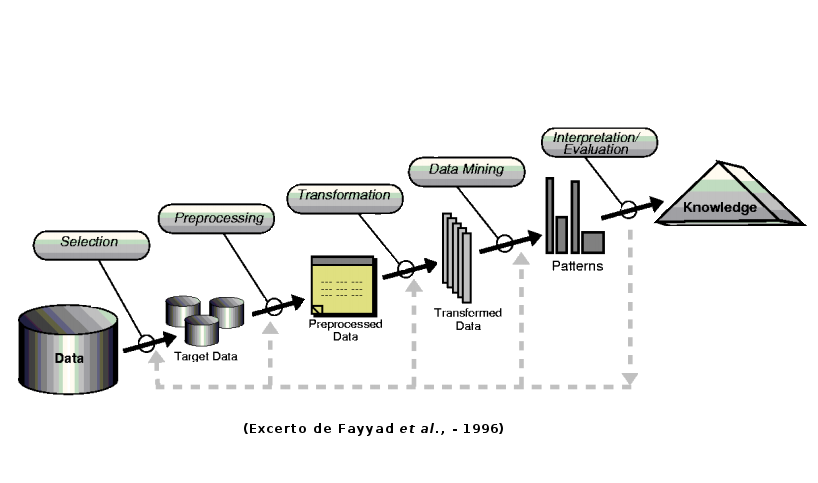
\includegraphics[width=90mm, height=75mm]{Figuras/FayyadSemFundo.png}
\end{figure}


O Big data está representado, na imagem, onde se lê ``Data'', repleto em dados ausentes e/ou inconsistentes por isso conhecidos como dados não estruturados. Os balão onde se lê ``Selection'' representa a coleta das informações, para este artigo representa a seleção dos dados no Big Data vindos das mais diversas fontes, tais como, redes sociais, câmaras de trânsito, informações de satélites meteorológicos e muitas outras fontes. Armazenar qualquer quantidade de dados nessa etapa pode ser um grande problema, devido a quantidade, como mencionado anteriormente, porém os dados relevantes podem ser armazenados em ``Target Data'' com Hadoop e as técnicas de ``Map'' e ``Reduce'' poder-se-ia agrupar (clustering) informações ou ler os fluxos de dados (stream data) algumas técnicas de IA podem ser aplicadas nessa etapa, como ``Data Mininng Swarm Robotics'' através de Botnets e ``Swarm Intelligence''. No balão ``Preprocessing'' ainda são dados não-estruturados, para estruturá-los é preciso técnicas linguísticas pois existe lógica entre eles \cite{Aranha2006}. Esses dados normalmente são coletados por técnicas de Mineração de Textos ou Mineração de Dados em Textos, mais uma vez técnicas de IA como ``Machine Learning'' como será descrito mais adiante. Uma vez transformados os dados em ``Transformation'' esses dados, já estruturados podem ser armazenados em Bancos de Dados conhecidos como Datawarehouse a exemplo do Hive, descrito na Figura 4. O processo de Mineração dos dados começa no balão ``Data Mining''. Nessa etapa são aplicados outros técnicas de IA como ``Decion Tree'', ``Artificial Neural Network'', ``Logistic Regression'', ``Deep Learning'' e muitas outras técnicas de classificação e extração de padrões. Todas essas etapas, na mineração de dados são recorrentes como indicam as setas pontilhadas. Algumas técnicas de mineração de dados são fortemente influenciadas pelas informações à entrada, como as Árvores de decisão ou ``Decision Tree'' \cite{DecisionTree} e Redes Neurais para minerar dados teriam milhares de neurônios na camada intermediária o que inviabilizaria a técnica aplicada a este contexto, portanto utilizar essas duas técnicas, para extrair informações do Big data, pode levar a inconsistências incontornáveis.

\vspace{0.1cm}

Utilizar técnicas de mineração de dados é para além de extrair dados, extrair conhecimento do negócio que se está analisando e com isso poder predizer os resultados futuros à saída do modelo, aquando determinados dados à entrada ocorrem. \cite{Amin2015}, essa técnica de extração de conhecimento chama-se \textit{Knowledge Discovery Databases} (KDD).


\subsection{Data Mining - Big Data}\label{arte:palavraChave:DataMiningBigData}

Minerar dados no Big data pode não ser uma tarefa atômica, devendo ser divida entre vários tarefas com vários processos em cada uma delas, como descrito anteriormente, pois os dados coletados até chegar a etapa de análise precisam ser tratados. Extrair conhecimento dos dados não processados não faz sentido, tratá-los só ``per si'' exige muito trabalho de IA como Mineração de dados em textos. Mineração em textos é inspirado em técnicas de ``Machine Learning'' \cite{Aranha2006}. Contudo analisar textos é basicamente entender o significado do texto, baseado em regras de associação lógica, o mapa mental a seguir mostra um modelo de análise de texto feito por seres humanos.

\begin{figure}[!ht]
\centering
\caption{Mapa mental de análise de textos}
\flushleft
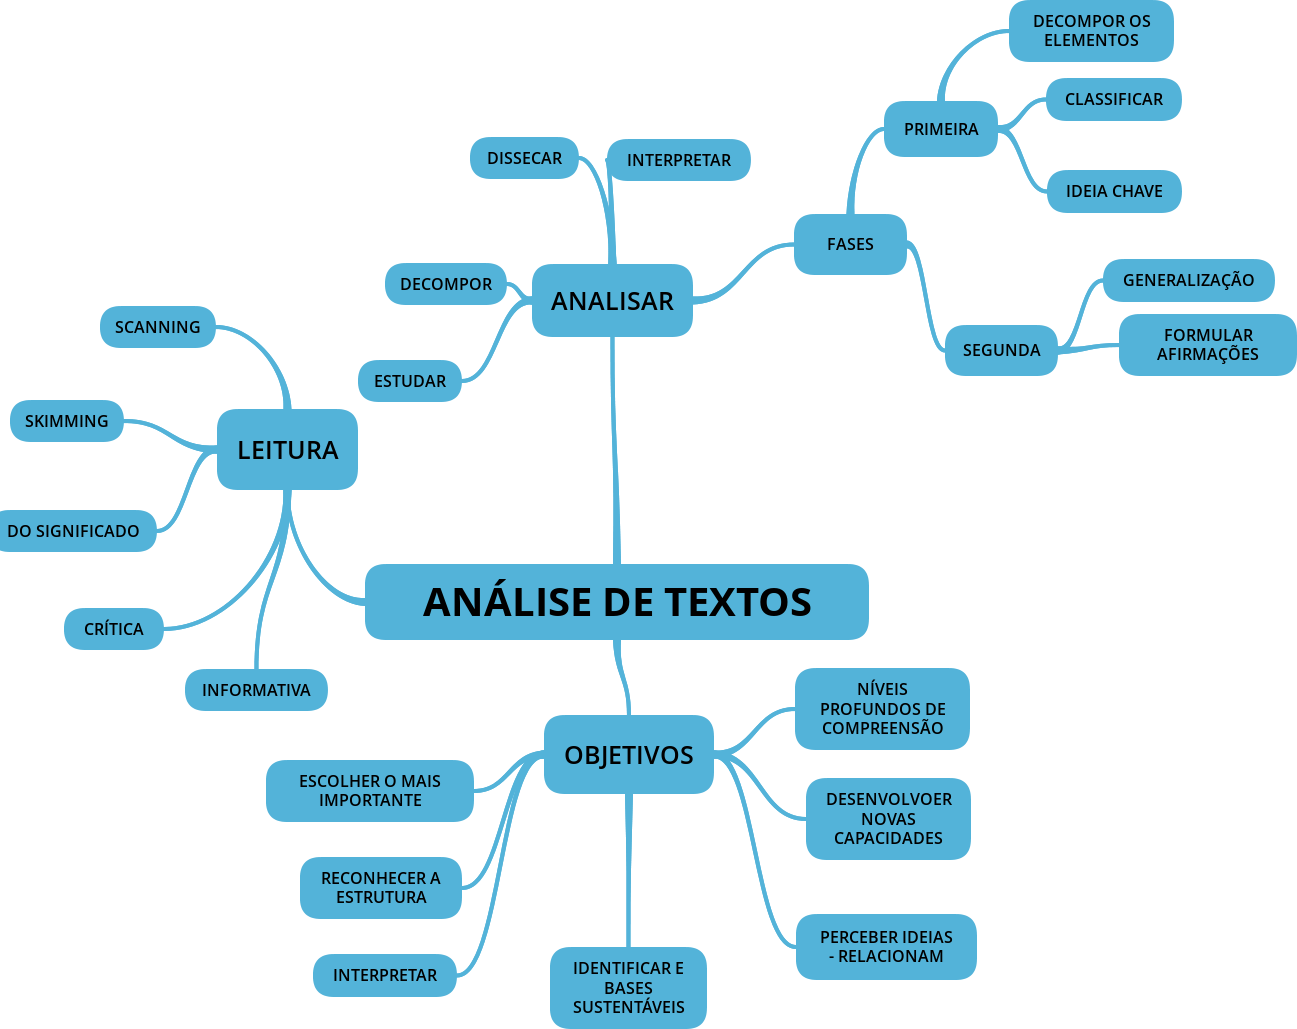
\includegraphics[width=90mm, height=60mm]{Figuras/Analise_Textos.png}
\end{figure}

Existem diversos técnicas algorítmicas para isso. No entanto todas elas necessitam que os dados sejam checados e validados constantemente, essa técnica é conhecida como ``CRoss Indrustry Standard Process for Data Mining'' (CrIP-DM). A figura a seguir exemplifica.

\begin{figure}[!ht]
\centering
\caption{Minerando dados no Big Data}
\flushleft
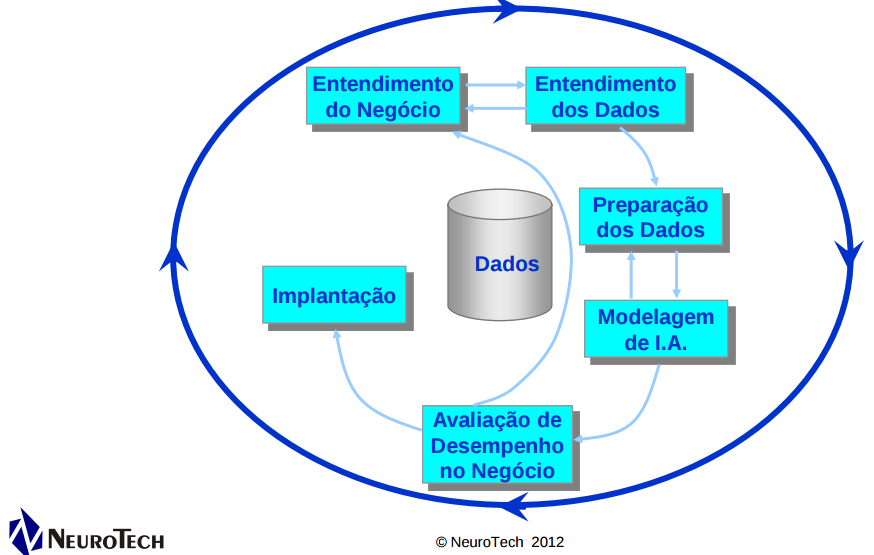
\includegraphics[width=70mm, height=60mm]{Figuras/CrispDM.png}
\end{figure}

O \textbf{Entendimento do negócio} é uma fase crucial da mineração, onde um especialista (ou muitos) deve ser consultado, pois o analista de dados geralmente consegue fazer re-uso de conhecimento lendo periódicos e artigos, mas o especialista no negócio é um profissional essencial e deve estar com anos de experiência no negócio.
Passada essa fase de Entendimento do Negócio o analista de dados poderá passar a fase do \textbf{Entendimento dos dados}, nesta fase o analista de dados ``olha'' para os dados com acurácia procurando identificar a qualidade dos dados. Dados ausentes são comuns em bancos de dados não estruturados, os``missing data'' são sempre um problema a ser considerado, pode consumir muito tempo do analista de dados. 
Após superar a fase do entendimento do negócio o analista de dados passará a fase da \textbf{Preparação dos dados}, esta fase cobre a construção final do conjunto de dados, preparar os dados significa criar selecionar atributos criar tabelas e registros dos dados. 
Na fase de \textbf{Modelagem de I.A.} a tecnologia deve ser escolhida com critério baseado em experiência do analista de dados. Em sistemas que exijam apoio a decisão uma tecnologia inadequada pode levar a decisões erradas, é comum retornar as fases anteriores para se adequar `as técnicas aos dados, por exemplo um modelo de regressão logística para problemas binários andam juntos na maioria dos sistemas, redes neurais andam juntos com problemas de classificação e assim por diante, contudo sempre há espaço para novas tecnologias e sobre tudo hibridização nas tenologias. ver figura a seguir:

\begin{figure}[!ht]
\centering
\caption{Modelo de IA baseado em ``Decision Tree'' para o Big Data}
\flushleft
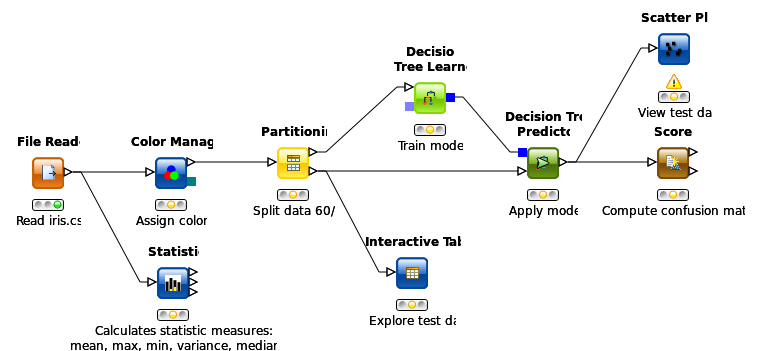
\includegraphics[width=90mm, height=50mm]{Figuras/workflow.png}
\end{figure}

Um conjunto de treinamento de ser preparado na fase anterior, para se fazer testes aos algorítimos dos Modelos de IA, contudo isso somente serve para se medir o acerto e a acurácia do modelo utilizado.

Métricas deverão ser propostas na fase de avaliação de desempenho pois minerar dados com poucos registros (< 10.000) não costumam construir bons sistemas suporte a decisão baseados em de mineração de dados.
\textbf{Avaliação de desempenho} em mineração de dados um ou muitos modelos devem ter sido construídos e testados e com alta qualidade da perspectiva da analise  dos dados.
Criar um modelo geralmente não é o fim do negócio, contudo é criar um modelo de entendimento do negócio. Até que se obtenha as respostas satisfatórias o modelo deverá ser refeito várias vezes até sua \textbf{Implantação}. A imagem a seguir descreve o domínio das técnicas aplicadas à mineração de dados:

\begin{figure}[!ht]
\centering
\caption{Domínio das técnicas aplicadas a mineração de dados}
\flushleft
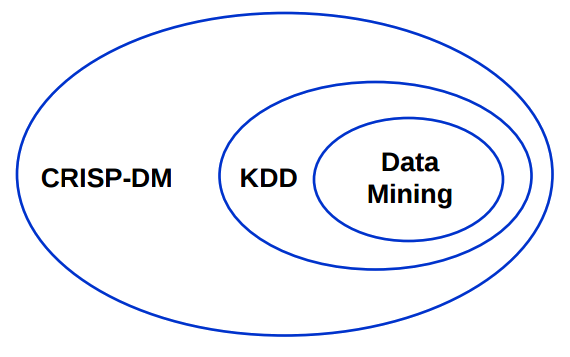
\includegraphics[width=90mm, height=50mm]{Figuras/RelacaoCrispKddDm.png}
\end{figure}



\section{Meta-heurísticas}


As meta-heurísticas são soluções encontradas nas mais diversas espécies de seres vivos, por exemplo, as formigas quando 
vão em busca de alimentos, facilmente encontram um caminho mais curto entre o ninho e a fonte de alimentos, cardumes de peixes 
executam movimentos aparentemente aleatórios mas, quando em grupo, são precisos para fuga dos predadores, bandos de pássaros 
quando em busca de novos locais para ninhos ou de alimento, inspiram os mais diversos algoritmos inteligentes baseados em 
populações de animais sociáveis, demonstrando que há uma inteligência coletiva nessas populações, desenvolvida ao longo do 
tempo e das interações entre essas espécies sociáveis e o meio ambiente. Essa classe de algoritmos, metaforiza o comportamento 
de tais populações, e promoveu o desenvolvimento de uma área que hoje é conhecida como computação bio inspirada ou computação 
natural. Essa área investiga a relação entre a computação e a biologia (e mesmo a sociologia), estudando soluções de buscas 
e otimização, modelando problemas mais eficientemente, baseado nas elegantes soluções encontradas pela natureza.


\section{Enxame de partículas}\label{arte:enxames}

Em 1989, G. Beni e J. Wang cunharam a expressão \textit{Swarm Intelligence}, no seu
trabalho em Robotic Swarm \cite{SRobotics}. O estudo do reino animal aprofundou-se no estudo
comportamental e possibilitou o melhor entendimento de como cooperam indivíduos dentro de um grupo e
quais os mecanismos usados para controlar o enxame e condicionar o indivíduo, tais como a estigmergia. 
Por enxame, pode entender-se manada, alcateia, bando, colônia, entre outras designações conforme o animal 
ou inseto e, a partir daqui, qualquer referência a um grupo de agentes passa a ser feita por enxame, e.g., 
um enxame de pássaros. Os 5 princípios da inteligência de enxame segundo  Chambers \cite{chambers2014computer}, são:
\begin{itemize}
	\item{Proximidade: os agentes têm que ser capaz de interagir}
	\item{Qualidade: os agentes devem ser capazes de avaliar seus comportamentos}
	\item{Diversidade: permite ao sistema reagir a situações inesperadas}
	\item{Estabilidade: nem todas as variações ambientais devem afetar o comportamento de um agente}
	\item{Adaptabilidade: capacidade de se adequar as variações ambientais}
\end{itemize}

\vspace{0.3cm}
\textbf{Swarm Optimization - (PSO)}
\vspace{0.1cm}

Kennedy e Eberhart (1995), criaram a popular Otimização por Enxame de Partículas do inglês \textit{Particle Swarm Optimization} - (PSO), 
que na verdade é uma técnica de otimização de funções não-lineares baseado em populações. Foi inspirado no comportamento
social em bando de pássaros, essa técnica é uma das mais conhecidas e investigadas hoje \cite{Kennedy1995}.
Esse algoritmo (e todos os outros) têm um fator de convergência, para fazer com que encontre mais rapidamente a resposta procurada.
Para acontecer isso foi introduzido um ''poleiro'' virtual. Com essa simples abordagem foi inaugurado uma nova
família de algorítimos baseados em enxames. 

No PSO, a população é chamada enxame e os indivíduos, partículas. Cada partícula se move no espaço de busca, 
à procura de regiões promissoras; cada partícula dessas representa uma solução candidata a resolver nosso problema.
A equação utilizada para encontrar uma partícula no espaço de busca foi emprestada da cinemática:

\begin{equation}
x_i(t+1) = x_i(t) + v_i(t+1)
\end{equation}

Onde $x_1(t)$ é a posição da partícula num determinado momento ``t''. O $x_i(t+1) $ é a posição atual da partícula.

A velocidade da partícula é de acordo com a equação:

\begin{equation}
	v_i(t+1) = v_i(t) + Nbest + Lbest
\end{equation}

$Nbest = c_1r_1j(t)[Nbest - x_i(t)]$

$Lbest = c_2r_2j(t)[Lbest - x_i(t)]$
\vspace{0.2cm}

Onde $v_i(t)$ é a velocidade num momento ''t'' qualquer e $v_i(t+1)$ é a velocidade atual da partícula.
Os coeficientes $c_1r_1j(t)$ e $c_2r_2j$ são números que variam entre 0 e 1 para mudar a posição da partícula.
O coeficiente $Nbest - x_i(t)$ é a melhor posição da partícula na vizinhança e $Lbest - x_i(t)$ é a melhor posição
numa região que engloba essa vizinhança.


\vspace{0.3cm}
 \textbf{Fish School Search - (FSS)}
\vspace{0.1cm}


Para contornar o problema explosão combinatória Carmelo e Buarque propuseram a meta-heurísticas da busca por cardume de peixes
ou o \textit{Fish School Search} - (FSS) \cite{Filho2008}.

Na busca FSS, cada peixe representa uma possível solução do problema.
Em busca por enxame de partículas há o problema da degradação do enxame, quando aparentemente as partículas encontram
um mínimo local (poderia ser máximo - depende da natureza do problema) ''pensando'' terem encontrado o mínimo global.
Para contornar esse problema da degradação do enxame introduz-se operadores que façam com que o exame saia desses ''fossos''
de busca.
O FSS possui operadores para evitar o problema da perda de qualidade, dentre esses podemos citar o operador de volatilidade, 
que faz com que o enxame expanda quando o enxame se concentra por muito tempo.

A equação que faz isso é a seguinte:

\begin{equation}
Bari(t) = \frac{\sum_{i=1}^{N}x_i(t)W_1(t)}{\sum_{i=1}^{N}x_i(t)}
\end{equation}


\vspace{0.3cm}
\textbf{Ant Colony Optimization - (ACO)}
\vspace{0.1cm}

A optimização por colônia de formigas ou \textit{Ant Colony Optimization} - (ACO) é uma técnica de otimização que foi
introduzida desde os anos 90's \cite{Blum2005} baseado no comportamento forrageiro de colônia de formigas.
O comportamento forrageiro em diversas espécies \cite{Dorigo2005} é objeto de estudo das ciências biológicas pois os animais predadores 
procuram otimizar seu ganho de proteína, ao comer sua presa, minimizando o gasto de energia, ou minimizando o esforço para
caçar, capturar e comer essa presa. Esse comportamento é explorado pelo ACO para buscar soluções aproximadas para um
problema de otimização discreto, para problemas de otimização contínuos e para problemas de roteamento em telecomunicações.

No caminho da busca por alimentos as formigas deixam no ambiente uma marca chamado de feromônio.
Esse feromônio evapora com o passar do tempo, sendo assim, a medida que mais formigas sigam um determinado caminho,
mais intenso o feromônio se fará presente. 

A equação da evaporação do feromônio no ambiente é segundo a fórmula:

\begin{equation}
p(i,j)= \frac{[\tau (i,j)]^{\alpha }.[\eta (i,j)]^{\beta}}{\sum [\tau (i,j)]^{\alpha }.[\eta (i,j)]^{\beta}}
\end{equation}



\subsection{Data Mining - Swarm Intelligence}\label{arte:palavraChave:Swarm}

Recentemente algorítimos de classificação baseados em ``Ant Colony Optimization'' (ACO) tem sido experimentado em mineração de dados\cite{Baig2012} o AntMiner é um deles.

O algorítimo AntMiner utiliza as formigas para gerar regras de classificação. Inicia com regra vazia e incrementalmente adiciona regras, uma de cada vez. A adição de cada termos é probabilística e baseada em dois fatores: a qualidade heurística do termo e a quantidade de feromônio depositado anteriormente pelas formigas. Após a parte antecedente da regra ser construída a parte consequente da regra é assinalada por maior votação da amostra de treinamento coberta pela regra. A regra é construída com podas aos termos irrelevantes para melhorar a acurácia do algorítimo. A qualidade da regra construída é determinada e o valor do feromônio é atualizado na trilha pela formiga, proporcional a qualidade da regra. Quando todas as formigas construírem as regras delas as melhores regras são selecionadas, colocadas numa lista de regras descobertas. A amostra de treinamento corretamente classificada pela regra são removidas do conjunto de treinamento. Esse processo é continuado até que o número de amostras não cobertas é pequeno e o usuário estabeleça um limiar. O produto final é uma lista de regras ordenadas que será usada para classificar um conjunto de testes. A seguir o algoritmo de classificação AntMiner:

\begin{algorithm}
	\SetAlgoLined
	\Entrada{$conjTreino = \{todosCasosTreinamento\};$}  
	\Saida{$DescobrirListaRegras = [];$}
	\Inicio{
		\Enqto{$conjTreino > MaxNaoDescoberto$}{
	 	{$ t = 1$ /*índice de formmigas*/ \\}  
	 	{$ j = 1$ /*índice de convergência*/\\}
	 	/*inicializa todas as trilhas com algum feromônio*/\\
	 		\Repita{$t>= No_ants$ ou $j >= NoRegrasConverg$}{
	 		 $Ant_t$ /*inicializa com regras em branco e incrementalmente constrói 					um classificados de regras $R_t$ por adição de termos um a um para as 				regras correntes; */\\
	 		 Podar regras $R_t;$
	 		 Atualizar o feromônio de todas as trilhas incrementando o feromônio na trilha de cada $Ant_t$ (proporcional à qualidade do $R_t$) e decrementa o feromônio em outras trilhas (simulando a evaporação de feromônio)
	 		 \Se{$R_t == R_t-1$ /*atualiza a convergência de testes*/\\}{
	 		 $j = j+1;$\\
	 		 \Senao{$j = 1;$}
	 		 }
	 		 $t = t+1;$
	 		 }
	 		 Escolher melhor regra $R_bost$ entre todas as regras $R_t$ construída pelas formigas;
	 		 Adicione regras $R_{bost}$ para $DescobrirListaRegras;$
	 		 $conjTreino$ = $conjTreino$ - \{casos correntes cobertos por $R_{bost}$\};
	 	}
 	 }
   \label{alg1}
   \caption{\textsc{Ant-Miner}}
\end{algorithm}


\subsection{Data Mining - Swarm Robotics}\label{arte:palavraChave:Robotics}

O rápido crescimento da Internet, tem trazido, a reboque, o contínuo crescimento da insegurança nos computadores e sistemas atuais \cite{Barford2007}.
Ataques utilizando a computadores através de robôs conhecidos como Botnet é um problema contante para que lida com segurança da informação. No entanto os Botnet podem ter uma vida mais digna, como coletar informações no Big data. O Google se especializou nisso quando utiliza seus ``Spiders''. Esses robôs navegam pela Internet ``devorando'' página e indexando-as para que as buscas do motor de buscas da Google seja mais eficiente. A figura a seguir podemos ver um exemplo desses robôs: \cite{motorBusca}

\begin{figure}[!ht]
\centering
\caption{Minerando textos no Big Data com robôs}
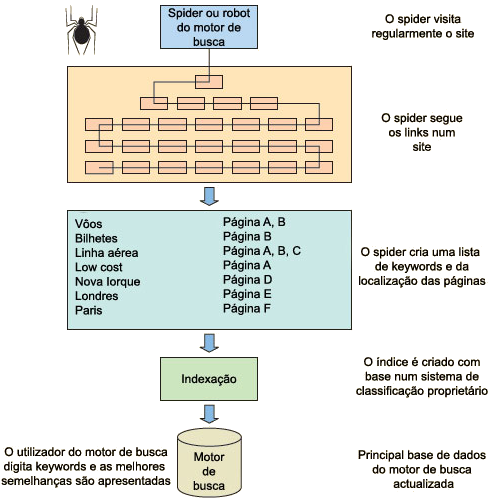
\includegraphics[width=60mm, height=60mm]{Figuras/Motordebusca.png}
\end{figure}

A utilização desses robôs é uma alternativa eficiente para coletar informações no Big data (ver ``Selection'' Figura 6) já que sua especialidade é essa. Como o Big data tem uma forte componente de inconsistência coletar informações das páginas visitas pelos robôs ou mesmo coletar a página inteira pode ser extremamente eficiente, nos quesitos ``volume'' e ``velocidade'' descrito na seção 6.1 (Hadoop -- Map Reduce -- Big Data). 


%\subsection{Deep Learning}\label{arte:palavraChave:Deep}



\subsection{Machine Learning}\label{arte:palavraChave:Machine}

O desafio \textit{Big Data} é resumido por alguns autoes a 3 V's (Velocidade, Variedade e Volume) dado que as informçãoes já tiveram um tratamento adequado (eliminando os últimos V's) contudo Velocidade, Variedade e Volume pode ser um fator determinístico na escolha da ferramenta mais adequada para se analisar dados do \textit{Big Data} e extrair informação. As árvores de decisão são algorimos rápidos, contudo dados impuros podem comprometer o desepenho desse algoritmo. A fase de extração dos dados do \textit{Big Data} são fortemente influenciáveis pelas variáveis escolhidas, \cite{DecisionTree} isso pode representar o desafio maior para implementar esta técnica, na figura a seguir exemplificamos essa tarefa:

%desenhar a figura

% \begin{tikzpicture}
%  \draw (0,0) -- (2,1); %reta
% \end{tikzpicture}






\section{Resultados esperados}

Este Survey têm diversos propósitos preliminares e também conclusivos, para balizar pesquisas na área, apontando um caminho mais promissor relacionado ao assunto escolhido, o Big Dada. Um dos propósito é servir de referência científica a qualquer de busca por conhecimento científico, mostrando o trabalho que o pesquisador deve ter, o cuidado ao procurar 
esse conhecimento, sem contaminar-se na ``floresta'' de artigos científicos, dissertações e teses ofertados e, disponíveis hodiernamente na Internet. 

Após a conclusão deste Survey, pretende-se incluir, os dados encontrados, no capítulo 2 da dissertação, servindo também de exemplo para todo mestrando que se aventurar na busca “indiscriminada” por artigos, deixando de lado uma parte importante do seu trabalho que são os dados estatísticos dessa fase e que pode ter assim uma abordagem científica já na fase inicial.
A fase conclusiva, desse Survey, será a certeza de que o melhor caminho escolhido para o desenvolvimento das outras fases da dissertação foi baseado em métodos científicos, desde sua fase inicial, ficando disponíveis para outros pesquisadores o ``como'' deve ser todo trabalho de busca por artigos científicos.


\section{Conclusão}

Devido à natureza da problemática ser as dimensões, o Big Data tem tornado-se um desfio hérculeo para quem envereda-se a desvendá-lo.
Inferir sobre o Big Data é o que muitos pesquisadores têm feito recentemente, utilizando-se para isso das mais diferentes tecnologias a disposição; Hadoop ou \textit{Map Reduce} ou uma combinação dos dois, essas fronteiras vêm sendo desmistificadas aos poucos, mas ao mesmo tempo, novos desafios se fazem presentes, com a chegada da Internet das Coisas, onde tudo está conectado \cite{madeira}
desde eletrodomésticos \cite{mayumi} a carros, sinais de trânsito, fazendo com que os \textit{smartphones} seja a ferramenta para se ter acesso a isso tudo. \cite{singer}
Portanto estamos só no começo, no que está por vir, fazendo com que haja cada vez mais trabalhos nessa área e inspirações para novos algoritmos.

% conference papers do not normally have an appendix



% use section* for acknowledgment
\ifCLASSOPTIONcompsoc
  % The Computer Society usually uses the plural form
  \section*{Acknowledgments}
\else
  % regular IEEE prefers the singular form
  \section*{Acknowledgment}
\fi


The authors would like to thank...



% references section

% can use a bibliography generated by BibTeX as a .bbl file
% BibTeX documentation can be easily obtained at:
% http://www.ctan.org/tex-archive/biblio/bibtex/contrib/doc/
% The IEEEtran BibTeX style support page is at:
% http://www.michaelshell.org/tex/ieeetran/bibtex/
%\bibliographystyle{IEEEtran}
% argument is your BibTeX string definitions and bibliography database(s)
%\bibliography{IEEEabrv,../bib/paper}
%
% <OR> manually copy in the resultant .bbl file
% set second argument of \begin to the number of references
% (used to reserve space for the reference number labels box)
\begin{thebibliography}{1}

%1
\bibitem{Forouzan}
FOROUZAN, Behrouz A. Comunicação de Dados e Redes de Computadores. São Paulo: McGraw-Hill, 2008

%2  
\bibitem{Swarm_Medeiros}
Talles Henrique De Medeiros, Luís Fabrício Wanderley Góes, M. B.-B. C. E. I. M. (n.d.). 
\emph{Computação Bioinspirada aplicada à Robótica}

%3
\bibitem{Specialski} 
E. ~SPECIALSKI (1999).
\emph{Gerência de redes de computadores e telecomunicações}

%4
\bibitem{bigdataQualquerUm}
  H. V. Jagadish, J. Gehrke, A. Labrinidis, Y. Papakontantinou, J. M. Patel, R. Ramakrishnan and C. Shahabi
  \emph{Exploring the inherent technical challenges in realizing the potential of Big Data},
  journal:Comunication of the ACM, volume=57, numbe=r7, pages=86--96, month=July, year=2014

%5
\bibitem{SRobotics}
H. ~Ahmed, and J. ~Glasgow,
\emph{Swarm intelligence: concepts, models and applications},
\relax School of Computing, Queen's University, Citeseer, 2012.

%6
\bibitem{singer}
SINGER, Talyta. TUDO CONECTADO: CONCEITOS E REPRESENTAÇÕES DA INTERNET DAS COISAS. 2012.
Acessado em: 23 abril. 2015.
\href{http://www.simsocial2012.ufba.br/modulos/submissao/Upload/44965.pdf} {Singer}

%7
\bibitem{Twitter2015}
Dorsey, J. Williams, B. Stone, E. and Glass, N.
Acessado em Julho de 2015
\href {https://pt.wikipedia.org/wiki/Twitter}
{Twitter}

%8
\bibitem{Filesystem}
Filho, João Heriberto Mota,
booktitle = {Descobrindo o Linux: entenda o sistema operacional GNU/Linux},
isbn = {978-85-7522-278-2},
pages = {153--162},
year = {2012}

%9
\bibitem{Conejero2015}
Conejero, Javier and Rana, Omer and Burnap, Peter and Morgan, Jeffrey and Caminero, Blanca and Carri{\'{o}}n, Carmen,
title = {{Analysing Hadoop power consumption and impact on application QoS}},
issn = {0167739X},
journal = {Future Generation Computer Systems},
mendeley-groups = {HadoopMapreduceinBigData},
doi = {10.1016/j.future.2015.03.009},
year = {2015}
\href{http://linkinghub.elsevier.com/retrieve/pii/S0167739X15000643}{HadoopMapreduce}


%10
\bibitem{Lange2015}
Lange, Benoit and Nguyen, Toan
title = {{A Hadoop use case for engineering data}},
mendeley-groups = {DataMiningBigData},
year = {2015}


%11
\bibitem{Dean2008}
Dean, Jeffrey and Ghemawat, Sanjay
institution = {Google, Inc.},
issn = {00010782},
journal = {Communications of the ACM},
number = {1},
pages = {1--13},
pmid = {11687618},
publisher = {ACM},
series = {SIGMOD '07},
title = {{MapReduce : Simplified Data Processing on Large Clusters}},
volume = {51},
year = {2008}
\href{http://portal.acm.org/citation.cfm?id=1327492}{MapReduce}


%12
\bibitem{Aranha2006}
Aranha, Christian and Passos, Emmanuel,
A Tecnologia de Mineração de Textos,
booktitle = {RESI-Revista Eletrônica de Sistemas de Informações},
doi = {10.5329/171},
issn = {1677-3071},
keywords = {Data minig,Intelligent information systems},
mendeley-groups = {Mineração Textos},
number = {2},
pages = {1--8},
volume = {2},
year = {2006}


%13
\bibitem{Amin2015}
Amin, Adnan and Faisal, Rahim and Imtiaz, Ali and Changez, Khan and Anwar, Sajid,
title = {{A Comparison of Two Oversampling Techniques (SMOTE vs MTDF) for Handling Class Imbalance Problem: A Case Study of Customer Churn Prediction}},
doi = {10.1007/978-3-319-16486-1},
isbn = {978-3-319-16485-4},
keywords = {big data,stock prediction,text mining},
mendeley-groups = {DataMiningBigData},
pages = {215--225},
volume = {353},
year = {2015},
\href{http://link.springer.com/10.1007/978-3-319-16486-1}{stockprediction}



%14
\bibitem{Barford2007}
Barford, Paul and Yegneswaran, Vinod,
title = {{An inside look at Botnets}},
doi = {10.1007/978-0-387-44599-1},
isbn = {978-0-387-32720-4},
issn = {03601315},
journal = {Malware Detection},
pages = {171--191},
volume = {27},
year = {2007}
\href{http://www.springerlink.com/index/10.1007/978-0-387-44599-1}{Botnet}


%17
\bibitem{Kennedy1995}
J. Kennedy and R. Eberhart (1995). 
\emph{Particle swarm optimization. In Neural Networks, 1995. Proceedings.}
IEEE International Conference on (Vol. 4, pp. 1942–1948 vol.4). http://doi.org/10.1109/ICNN.1995.488968

%18
\bibitem{Blum2005}
C. Blum
\emph{Ant colony optimization}
booktitle: {Physics of Life Reviews},
title: {{Ant colony optimization: Introduction and recent trends}},
doi: {10.1016/j.plrev.2005.10.001},
issn: {15710645},
keywords: {Ant colony optimization,Discrete optimization,Hybridization},
number: {4},
pages: {353--373},
volume: {2},
year {2005}

%19
\bibitem{Dorigo2005}
M. Dorigo and C. Blum,
\emph{Ant colony optimization theory: A survey},
doi: {10.1016/j.tcs.2005.05.020},
isbn: {0304-3975},
issn: {03043975},
journal: {Theoretical Computer Science},
keywords: {Ant colony optimization, Approximate algorithms, Combinatorial optimization, Convergence, Metaheuristics, Model-based search, Stochastic gradient descent},
number: {2-3},
pages: {243--278},
volume: {344},
year: {2005}

%20
\bibitem{Filho2008}
Filho, Carmelo J A Bastos and Neto, Fernando B De Lima and Lins, Anthony J C C and Nascimento, Ant\^{o}nio I S and Lima, Mar\'{\i}lia P.
booktitle: {Conference Proceedings - IEEE International Conference on Systems, Man and Cybernetics},
\emph{A novel search algorithm based on fish school behavior},
doi: {10.1109/ICSMC.2008.4811695},
isbn: {978-1-4244-2383-5},
issn: {1062922X},
keywords: {Fish school,Search algorithms,Social behaviour,Swarm intelligence},
pages: {2646--2651},
year: {2008}

%21
\bibitem{Baig2012}
Baig, Abdul Rauf and Shahzad, Waseem,
doi = {10.1007/s00521-010-0490-5},
title = {{A correlation-based ant miner for classification rule discovery}},
issn = {09410643},
journal = {Neural Computing and Applications},
keywords = {Ant colony optimization (ACO),Classification rules,Data mining,Swarm intelligence},
mendeley-groups = {DataMiningSwarnIntelligence},
number = {2},
pages = {219--235},
volume = {21},
year = {2012}


%14.1
\bibitem{motorBusca}
Fonte: Chaffey,
page = 378,
year=2006


%15
\bibitem{DecisionTree}
A. Srivastava, V. Katiyar and N. Singh -- Review of Decision Tree Algorithm: Big Data Analytics,
International Journal of Informative \& Futuristic Research,
number = {10},
pages = {3644--3654},
volume = {2},
year = {2015}

%16
\bibitem{chambers2014computer}
W. D. Chambers (2014).
\emph{Computer simulation of dental professionals as a moral community. Medicine, Health Care and Philosophy}
\relax  17(3), 467–476.




%22
\bibitem{madeira}
Madeira, Lamont. Hoje a internet, amanhã os desafios da internet das coisas. 2011.

%23
\bibitem{mayumi}
MAYUMI, Danielle. Computação nas nuvens – O futuro da internet. 2011.



\end{thebibliography}






% that's all folks
\end{document}


